% ─── Chapter 1: Introduction ─────────────────────────────────────────────────

\begin{frame}{Introduction \& Motivation}
  \begin{columns}[T]
    \begin{column}{0.48\textwidth}
      \begin{block}{Scope: Education \& Research}
        \footnotesize
        \begin{itemize}
          \setlength{\itemsep}{3pt}
          \item \textbf{Education}: Interactive physics in the browser. Zero install, instant feedback.
          \item \textbf{Research}: Pushing the limits of real-time model order reduction.
        \end{itemize}
      \end{block}
      
      \vspace{0.15cm}
      
      \begin{block}{Problem \& Solution}
        \footnotesize
        \begin{itemize}
          \setlength{\itemsep}{3pt}
          \item \textbf{The Goal}: Instant physics whenever geometry changes.
          \item \textbf{The Problem}: Standard FEM is too slow. Remeshing kills real-time.
          \item \textbf{The Solution}: Exact shapes with IGA, massive speed with ROM.
        \end{itemize}
      \end{block}
    \end{column}
    
    \begin{column}{0.48\textwidth}
      \centering
      \vspace*{0.85cm}
      \begin{tikzpicture}
        \begin{scope}
          \clip[rounded corners=5pt] (0,0) rectangle (5.5, 2.59);
          \node[anchor=south west, inner sep=0pt] at (0,0) {%
            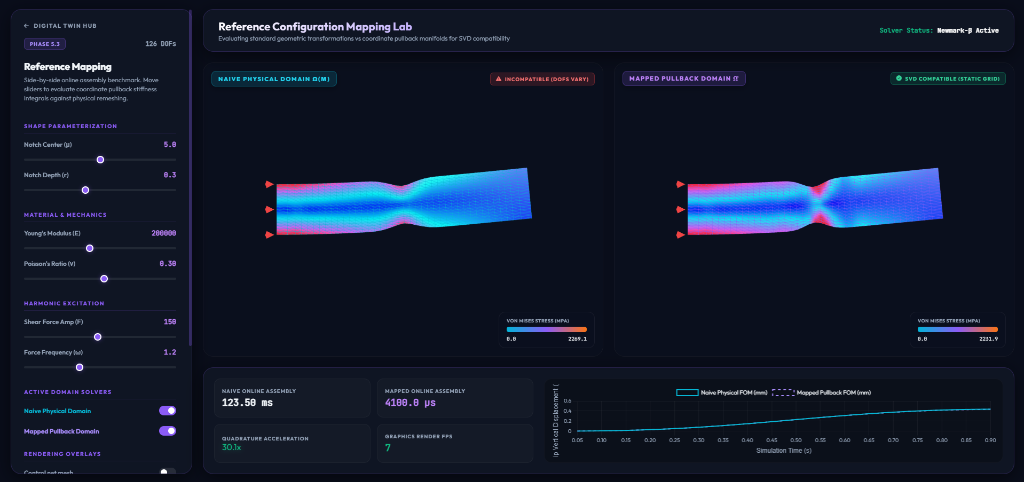
\includegraphics[width=5.5cm, height=2.59cm, keepaspectratio]{web_app_ui.png}%
          };
        \end{scope}
        \draw[rounded corners=5pt, cnamred!60, line width=1.0pt] (0,0) rectangle (5.5, 2.59);
      \end{tikzpicture}
      
      \vspace{0.35cm}
      {\small\href{https://cnam-internship-mumen.netlify.app/app/playground\#5.3a}{\beamergotobutton{Open Web Simulation}}}
    \end{column}
  \end{columns}
\end{frame}

% Slide: Conceptual Parallels
\begin{frame}{Conceptual Parallels to Data Compression}
  \begin{columns}[T]
    % Column 1: IGA
    \begin{column}{0.31\textwidth}
      \begin{block}{\centering IGA \hfill \tiny [Hughes, 2005]}
        \centering
        \vspace{0.06cm}
        \begin{tikzpicture}
          \begin{scope}
            \clip[rounded corners=3pt] (0,0) rectangle (2.0, 3.0);
            \node[anchor=south west, inner sep=0pt] at (0,0) {%
              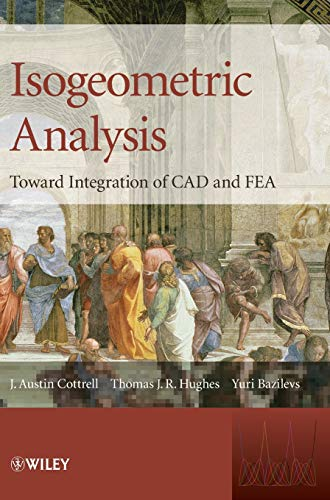
\includegraphics[width=2.0cm, height=3.0cm, keepaspectratio]{ref_iga_cottrell.jpg}%
            };
          \end{scope}
          \draw[rounded corners=3pt, cnamred!60, line width=0.8pt] (0,0) rectangle (2.0, 3.0);
        \end{tikzpicture}\\[0.08cm]
        {\tiny\textbf{Cottrell, Hughes, Bazilevs}}\\[0.04cm]
        {\scriptsize\color{black!75} Exact CAD geometry via NURBS without remeshing.}
      \end{block}
    \end{column}

    % Column 2: ROM
    \begin{column}{0.31\textwidth}
      \begin{block}{\centering ROM \hfill \tiny [Quarteroni, 2016]}
        \centering
        \vspace{0.06cm}
        \begin{tikzpicture}
          \begin{scope}
            \clip[rounded corners=3pt] (0,0) rectangle (2.0, 3.0);
            \node[anchor=south west, inner sep=0pt] at (0,0) {%
              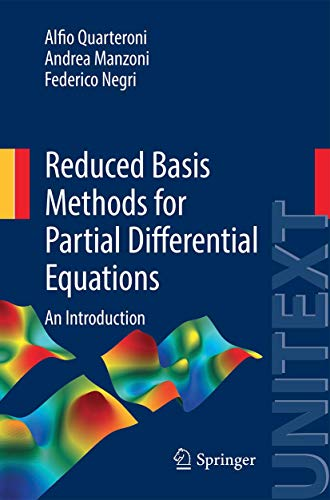
\includegraphics[width=2.0cm, height=3.0cm, keepaspectratio]{ref_quarteroni_rom.jpg}%
            };
          \end{scope}
          \draw[rounded corners=3pt, cnamred!60, line width=0.8pt] (0,0) rectangle (2.0, 3.0);
        \end{tikzpicture}\\[0.08cm]
        {\tiny\textbf{Quarteroni, Manzoni, Negri}}\\[0.04cm]
        {\scriptsize\color{black!75} Projection onto dominant modal subspaces ($r \ll N$).}
      \end{block}
    \end{column}

    % Column 3: Hyper-Reduction
    \begin{column}{0.31\textwidth}
      \begin{block}{\centering Hyper-ROM \hfill \tiny [Farhat, 2014]}
        \centering
        \vspace{0.06cm}
        \begin{tikzpicture}
          \begin{scope}
            \clip[rounded corners=3pt] (0,0) rectangle (2.0, 3.0);
            \node[anchor=south west, inner sep=0pt] at (0,0) {%
              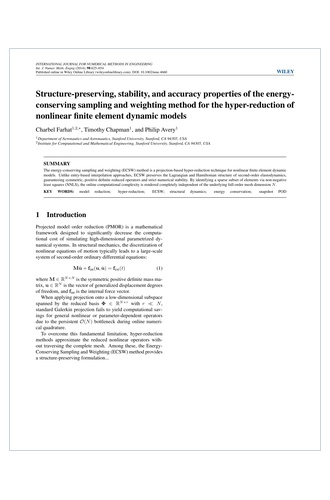
\includegraphics[width=2.0cm, height=3.0cm, keepaspectratio]{ref_farhat_paper_card.jpg}%
            };
          \end{scope}
          \draw[rounded corners=3pt, cnamred!60, line width=0.8pt] (0,0) rectangle (2.0, 3.0);
        \end{tikzpicture}\\[0.08cm]
        {\tiny\textbf{Farhat, Chapman, Avery}}\\[0.04cm]
        {\scriptsize\color{black!75} Energy-Conserving Sampling \& Weighting (ECSW).}
      \end{block}
    \end{column}
  \end{columns}
\end{frame}


